\documentclass[12pt]{article}

%===============================
%
%          📦 Paquetes
%
%===============================

\usepackage[a4paper, top=2cm, bottom=2cm, left=2.5cm, right=2.5cm]{geometry}
\usepackage[spanish]{babel}
\usepackage[utf8]{inputenc}
\usepackage{amsmath}
\usepackage{multicol}
\usepackage{graphicx}
\usepackage{hyperref}
\usepackage{booktabs}
\usepackage{pgfplots}
\pgfplotsset{compat=1.18}

\title{
  \vspace{2cm}
  \pagenumbering{gobble}
  
\includegraphics[width=5cm]{../assets/logo-utp.png} \\
  \vspace{1cm}
  \textbf{Universidad Tecnológica del Perú} \\
  \vspace{2cm}
  \textbf{Investigación Operativa} \\
  \vspace{1cm}
  \large \textbf{S04 - Ejercicios}
}
\author{
  \textbf{Torres Vara, Mateo Nicolas} - \texttt{U24308542} \\
  \texttt{Sección 36373}
}



\begin{document}
\maketitle
\begin{center}

  Docente: Alberto Andre Reyna Alcantara

\end{center}

%======================================
%
%          📚 Inicio del documento
%
%======================================

\newpage
\section*{Ejercicio 1}
\noindent Una empresa produce tres modelos de sillas diferentes, cada uno de estos modelos requiere una cantidad de madera y tela, la madera tiene un costo de 6 soles por cada pie y la tela tiene un costo de 4 soles por metro cuadrado. Además, cada modelo requiere de horas de trabajo de mano de obra en los departamentos de producción, el departamento 1 tiene un total de 800 horas y el departamento 2 tienen una disponibilidad de 600 horas. \\
En la siguiente tabla se muestra la información necesaria para la producción, además del precio de venta para cada producto, así como la demanda máxima estimada que tiene cada producto.

\begin{center}
  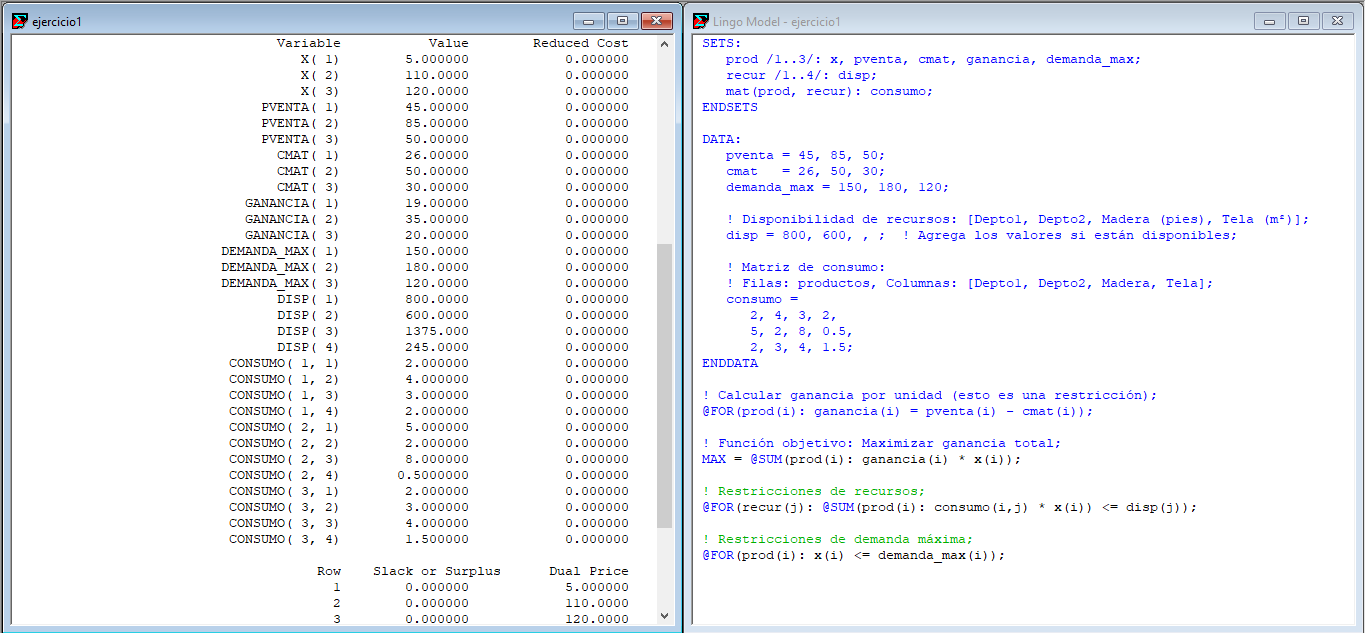
\includegraphics[width=1\textwidth]{./assets/ejercicio1.PNG}
\end{center}

\subsection*{Conclusión}
\noindent Basado en el módelo de programación lineal planteado, se concluye que para maximizar las ganancias, la empresa debe producir 5 unidades del modelo 1, 110 unidades del modelo 2 y 120 unidades del modelo 3.


\newpage
\section*{Ejercicio 2}
\noindent Una empresa tiene 3 máquinas para producir un mismo producto. La máquina N°1 tiene una tasa de producción de 20 unidades por hora mientras que la tasa de la máquina N°2 es de 40 unidades por hora, y la máquina N°3 tiene una tasa de producción de 30 unidades por hora. La máquina N°1 utiliza 40 kilos de materia prima por hora, la máquina N°2 utiliza 50 kilos por hora y la máquina N°3 utiliza 45 kilos de materia prima por hora. \\\\
El precio de venta de cada unidad del producto es de \$ 18. La máquina N°1 estará disponible a lo más 15 horas, la máquina N°2 a lo más 10 horas mientras que la máquina N°3 máximo estará disponible 12 horas. \\\\
Se cuenta con 1200 kilos de materia prima. El costo de la materia prima es de \$ 6 por kilo. Los costos de operación de las máquinas N°1, N°2 y N°3 son de \$ 50, \$70 y \$ 60 por hora respectivamente. Determinar la cantidad de horas que debe trabajar cada una de las tres máquinas para maximizar la utilidad total.

\vspace{0.5cm}

\begin{table}[!htbp]
  \centering
  \begin{tabular}{c c c c c}
    \toprule
       & \textbf{producción} & \textbf{material} & \textbf{costo producción} & \textbf{horas disp}\\
    \midrule
    M1 & 20 & 40 & 50 & 15 \\
    M2 & 40 & 50 & 70 & 10 \\
    M3 & 30 & 45 & 60 & 12 \\
    \midrule
    MAX & & 1200 & & \\
    \bottomrule
  \end{tabular}
  \caption{Datos de producción}
  \label{tab:ejercicio2}
\end{table}

\subsection*{Conclusión}
\noindent Basado en el módelo de programación lineal planteado, se concluye que para maximizar las ganancias, la empresa debe operar la máquina 1 por 4 horas, la máquina 2 por 10 horas y la máquina 3 por 12 horas.

\newpage
\section*{Recursos y créditos}

\begin{itemize}
    \item \textbf{Código fuente:} \href{https://github.com/MateoTVara/C08-InvestigacionOperativa}{Repositorio GitHub - Investigación Operativa}
    \item \textbf{Carátula por:} \href{https://github.com/1nfinit0}{1nfinit0 en GitHub}
\end{itemize}

\end{document}